\documentclass{article}
\usepackage[utf8]{inputenc}
\usepackage[T1]{fontenc}
\usepackage{lmodern}
\usepackage[brazil]{babel}
\usepackage{geometry}
\usepackage{graphicx}
\usepackage{float}
\usepackage{array}
\usepackage{booktabs}
\usepackage{amsmath}
\usepackage{hyperref}
\usepackage{listings}
\usepackage{xcolor}

\lstdefinestyle{mystyle}{
    language=C,
    backgroundcolor=\color{black!5},   
    commentstyle=\color{green!50!black},
    keywordstyle=\color{blue},
    numberstyle=\tiny\color{gray},
    stringstyle=\color{red},
    basicstyle=\ttfamily\footnotesize,
    breaklines=true,
    numbers=left,
    numbersep=5pt,
    frame=single,
    captionpos=b
}

\lstset{style=mystyle}

\title{Roteiro 1}
\author{Ana Beatriz Barbosa Yoshida - RA: 245609 \\ Julio Nunes Avelar - RA: 241163}
\date{Agosto de 2025}

\begin{document}

\maketitle

\tableofcontents
\newpage

% ---------------- Experiência 1 ----------------
\section{Experiência 1}

\subsection{Identificação das GPIOs do LED RGB}
\textbf{Pergunta:} Identifique as GPIOs que estão conectadas no LED RGB da BitDogLab. \\

\noindent
\textbf{Resposta:} As conexões do LED RGB com resistores de proteção estão descritas a seguir:  
\begin{itemize}
    \item Vermelho: GPIO 13 com resistor de 220 $\Omega$
    \item Verde: GPIO 11 com resistor de 220 $\Omega$
    \item Azul: GPIO 12 com resistor de 150 $\Omega$
\end{itemize}

\subsection{Níveis lógicos do RP2040}
\textbf{Pergunta:} Qual a tensão de saída de cada nível lógico do RP2040? \\

\noindent
\textbf{Resposta:} Os níveis lógicos do microcontrolador RP2040 são:  
\begin{itemize}
    \item Nível lógico 0: 0 V
    \item Nível lógico 1: 3.3 V
\end{itemize}

\subsection{Circuito básico e cálculo dos resistores}
\textbf{Pergunta:} Desenhe o circuito básico para acender este LED com as GPIOs. Calcule o valor de cada resistor. \\

\noindent
\textbf{Resposta:} O circuito básico do LED RGB está ilustrado na Figura \ref{fig:circuito_led}.  

\begin{figure}[H]
    \centering
    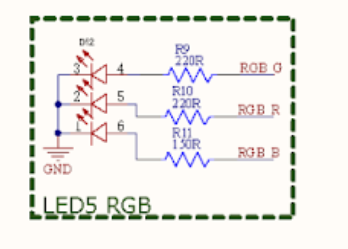
\includegraphics[width=0.6\textwidth]{circuito_led.png}
    \caption{Circuito do LED RGB com resistores.}
    \label{fig:circuito_led}
\end{figure}

O cálculo dos resistores é feito pela Lei de Ohm:  
\[
R = \frac{V_{CC} - V_{LED}}{I_{LED}}
\]

Os valores de corrente e tensão utilizados para cada cor do Led RGB podem ser encontrados no datasheet do Led

\subsection{Tarefa 1.1 -- Comparação entre linguagens}
\textbf{Pergunta:} Comparar o tempo de resposta e fluxo de execução entre C e MicroPython. Sugira um método para obter esses valores e crie uma tabela para realizarmos um Benchmark. \\

\noindent
\textbf{Resposta:}  
Para realizar o Benchmark entre as duas implementações (C e MicroPython), podemos analisar o tempo gasto para executar rotinas simples, como configuração de GPIOs, execução de funções básicas (acender um LED, imprimir uma string) e cálculos matemáticos. Os resultados obtidos estão apresentados na Tabela \ref{tab:benchmark}.  

\begin{table}[H]
    \centering
    \label{tab:benchmark}
    \begin{tabular}{lcc}
        \toprule
        Linguagem & Tempo ($\mu$s) & Teste \\
        \midrule
        C            & 13       & Inicialização das GPIOs \\
        MicroPython  & 452      & Inicialização das GPIOs \\
        C            & 10010890 & Loop com blink (10 iterações) \\
        MicroPython  & 10000689 & Loop com blink (10 iterações) \\
        C            & 246757   & Verificação de primos \\
        MicroPython  & 1226509  & Verificação de primos \\
        \bottomrule
    \end{tabular}
    \caption{Benchmark básico entre C e MicroPython.}
\end{table}

\subsection{Tarefa 1.2 -- Comparativo Imperativo vs OO}
\textbf{Pergunta:} Comparar tamanho do código (em bytes), tempo de resposta e fluxo de execução entre os modos imperativo e OO para ambos: MicroPython e C. Sugira um método para obter esses valores e crie uma tabela para realizarmos um Benchmark.  \\

\noindent
Uma comparação direta entre o tamanho das duas linguagens não é particularmente interessante, principalmente devido à grande diferença de paradigmas e formas de execução. A implementação em C gera um binário completo, contendo todas as instruções necessárias para o funcionamento do programa, enquanto a implementação em MicroPython gera um bytecode que é executado em uma máquina virtual (VM).

Por outro lado, comparar apenas o tamanho do código-fonte também não é adequado, pois depende fortemente da aplicação e do programador. Uma implementação simples em MicroPython tem grandes chances de ser menor que sua equivalente em C. No entanto, em casos que exigem acesso direto a registradores ou o uso de recursos específicos, a implementação em C é geralmente mais simples e eficiente.

De toda forma, a Tabela \ref{tab:benchmark_oo} apresenta um comparativo de tamanho de código, considerando, no caso do C, o tamanho do binário gerado (não o arquivo UF2), e, no caso do MicroPython, o tamanho do bytecode produzido.

A tabela \ref{tab:benchmark_oo}

\begin{table}[H]
    \centering
    \label{tab:benchmark_oo}
    \begin{tabular}{lcc}
        \toprule
        Paradigma & Linguagem & Tamanho Código (bytes) \\
        \midrule
        Imperativo & C        & 25K  \\
        OO         & C        & 25K  \\
        Imperativo & Python   & 259  \\
        OO         & Python   & 320  \\
        \bottomrule
    \end{tabular}
    \caption{Benchmark entre tamanho de código.}
\end{table}

% ---------------- Experiência 2 ----------------
\section{Experiência 2}

\subsection{GPIOs conectados aos botões}
\textbf{Pergunta:} Identifique as GPIOs que estão conectadas aos 3 botões.  

\textbf{Resposta:}  
A identificação está apresentada na Tabela \ref{tab:botoes}.  

\begin{table}[H]
    \centering
    \begin{tabular}{ccc}
        \toprule
         Botão & IO   & Função \\
         \midrule
         RESET  & RUN  & Reset do Pi Pico \\
         Botão A & GP05 & Botão genérico \\
         Botão B & GP06 & Botão genérico \\
         Botão C & GP10 & Botão genérico \\
        \bottomrule
    \end{tabular}
    \caption{Mapeamento dos botões conectados ao RP2040.}
    \label{tab:botoes}
\end{table}

\subsection{Limites de tensão para nível lógico}
\textbf{Pergunta:} Quais os limites de tensão considerados como nível baixo e alto no microcontrolador utilizado? \\ 

\textbf{Resposta:}  
\begin{itemize}
    \item Nível baixo: $V < V_{IL(max)}$
    \item Nível alto: $V > V_{IH(min)}$
\end{itemize}

Com $V_{IL(max)}$ sendo 0.8V e $V_{IH(min)}$ sendo 2.0V.

\subsection{Esquema dos botões}
\textbf{Pergunta:} Represente como os botões estão conectados ao microcontrolador.  \\

\noindent
\textbf{Resposta:}  
O esquema está mostrado na Figura \ref{fig:circuito_botoes}.  

\begin{figure}[H]
    \centering
    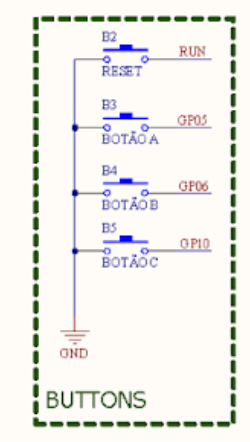
\includegraphics[width=0.6\textwidth]{circuito_botoes.png}
    \caption{Conexão dos botões ao RP2040.}
    \label{fig:circuito_botoes}
\end{figure}

\subsection{Debounce, Polling e IRQ}

\begin{table}[H]
    \centering
    \begin{tabular}{lcccccc}
        \toprule
         Método & Carga(N) & Nº de alternâncias do LED & Perdas & Latência & Observação\\
         \midrule
         Polling & 0 & 10 & 0 & 0 & \\
         Polling & 2k & 10 & 0 & 0 & \\
         Polling & 8k & 10 & 0 & 0 & \\
         Polling & 32k & 6 & 4 & 1 & \\
         Polling & 128k & 1 &  9 & 3 & \\
         \bottomrule
    \end{tabular}
    \caption{Tabela de teste de polling para 10 cliques}
    \label{tab:polling_compair}
\end{table}

\begin{table}[ht!]
    \centering
    \begin{tabular}{lcccccc}
        \toprule
         Método & Carga(N) & Nº de alternâncias do LED & Perdas & Latência & Observação\\
         \midrule
         IRQ & 0 & 10 & 0 & 0 & \\
         IRQ + Carga & 32k & 10 & 0 & 0 & \\
         \bottomrule
    \end{tabular}
    \caption{Tabela de teste de IRQ para 10 cliques}
    \label{tab:irq_compair}
\end{table}

\noindent
\textbf{Pergunta (Funcionalidade):} Confirme se o LED alternou a cada toque nos dois modos (Polling e IRQ), com debounce funcionando. \\

\noindent
Ele alternou em ambos.   \\ 


\noindent
\textbf{Pergunta (Latência):} Descreva o efeito de aumentar a “carga” no laço do Polling e compare com o comportamento no modo IRQ. \\

\noindent
O aumento da carga no modo Polling provoca maior latência, enquanto o uso de IRQ garante resposta mais imediata.   \\

\noindent
\textbf{Pergunta (Consumo de energia):} Argumente por que o método baseado em IRQ tende a ser mais eficiente em consumo de CPU e energia. Utilize as observações feitas durante o experimento. \\

\noindent
O IRQ é mais eficiente, pois evita que a CPU fique em espera constante. \\

\noindent
\textbf{Pergunta (Aplicações):} Quando usar o quê? \\

\noindent
Polling pode ser suficiente em sistemas simples (ex.: leitura periódica de sensores), enquanto IRQ é essencial em sistemas críticos (ex.: teclados, comunicações seriais).  \\

\subsection{Tabela Comparativa -- Polling × IRQ}
A Tabela \ref{tab:polling_irq} resume a comparação entre Polling e IRQ.  

\begin{table}[H]
    \centering
    \begin{tabular}{lcc}
        \toprule
        Critério & Polling & IRQ \\
        \midrule
        Latência percebida & Maior & Menor \\
        Perdas de eventos  & Possível & Improvável \\
        Consumo de CPU     & Elevado & Reduzido \\
        Complexidade       & Baixa  & Maior \\
        Situações suficientes & Sistemas simples & --- \\
        Situações obrigatórias & --- & Sistemas críticos \\
        \bottomrule
    \end{tabular}
    \caption{Comparativo entre Polling e IRQ.}
    \label{tab:polling_irq}
\end{table}

% ---------------- Experiência 3 ----------------
\section{Experiência 3}

\subsection{Fluxograma}
\noindent
\textbf{Pergunta:} Fluxograma do programa (laço → leitura → detecção de borda → toggle → aplicar LEDs). \\

\noindent
O digrama está presente na Figura \ref{fig:togle}. \\

\begin{figure}[ht!]
    \centering
    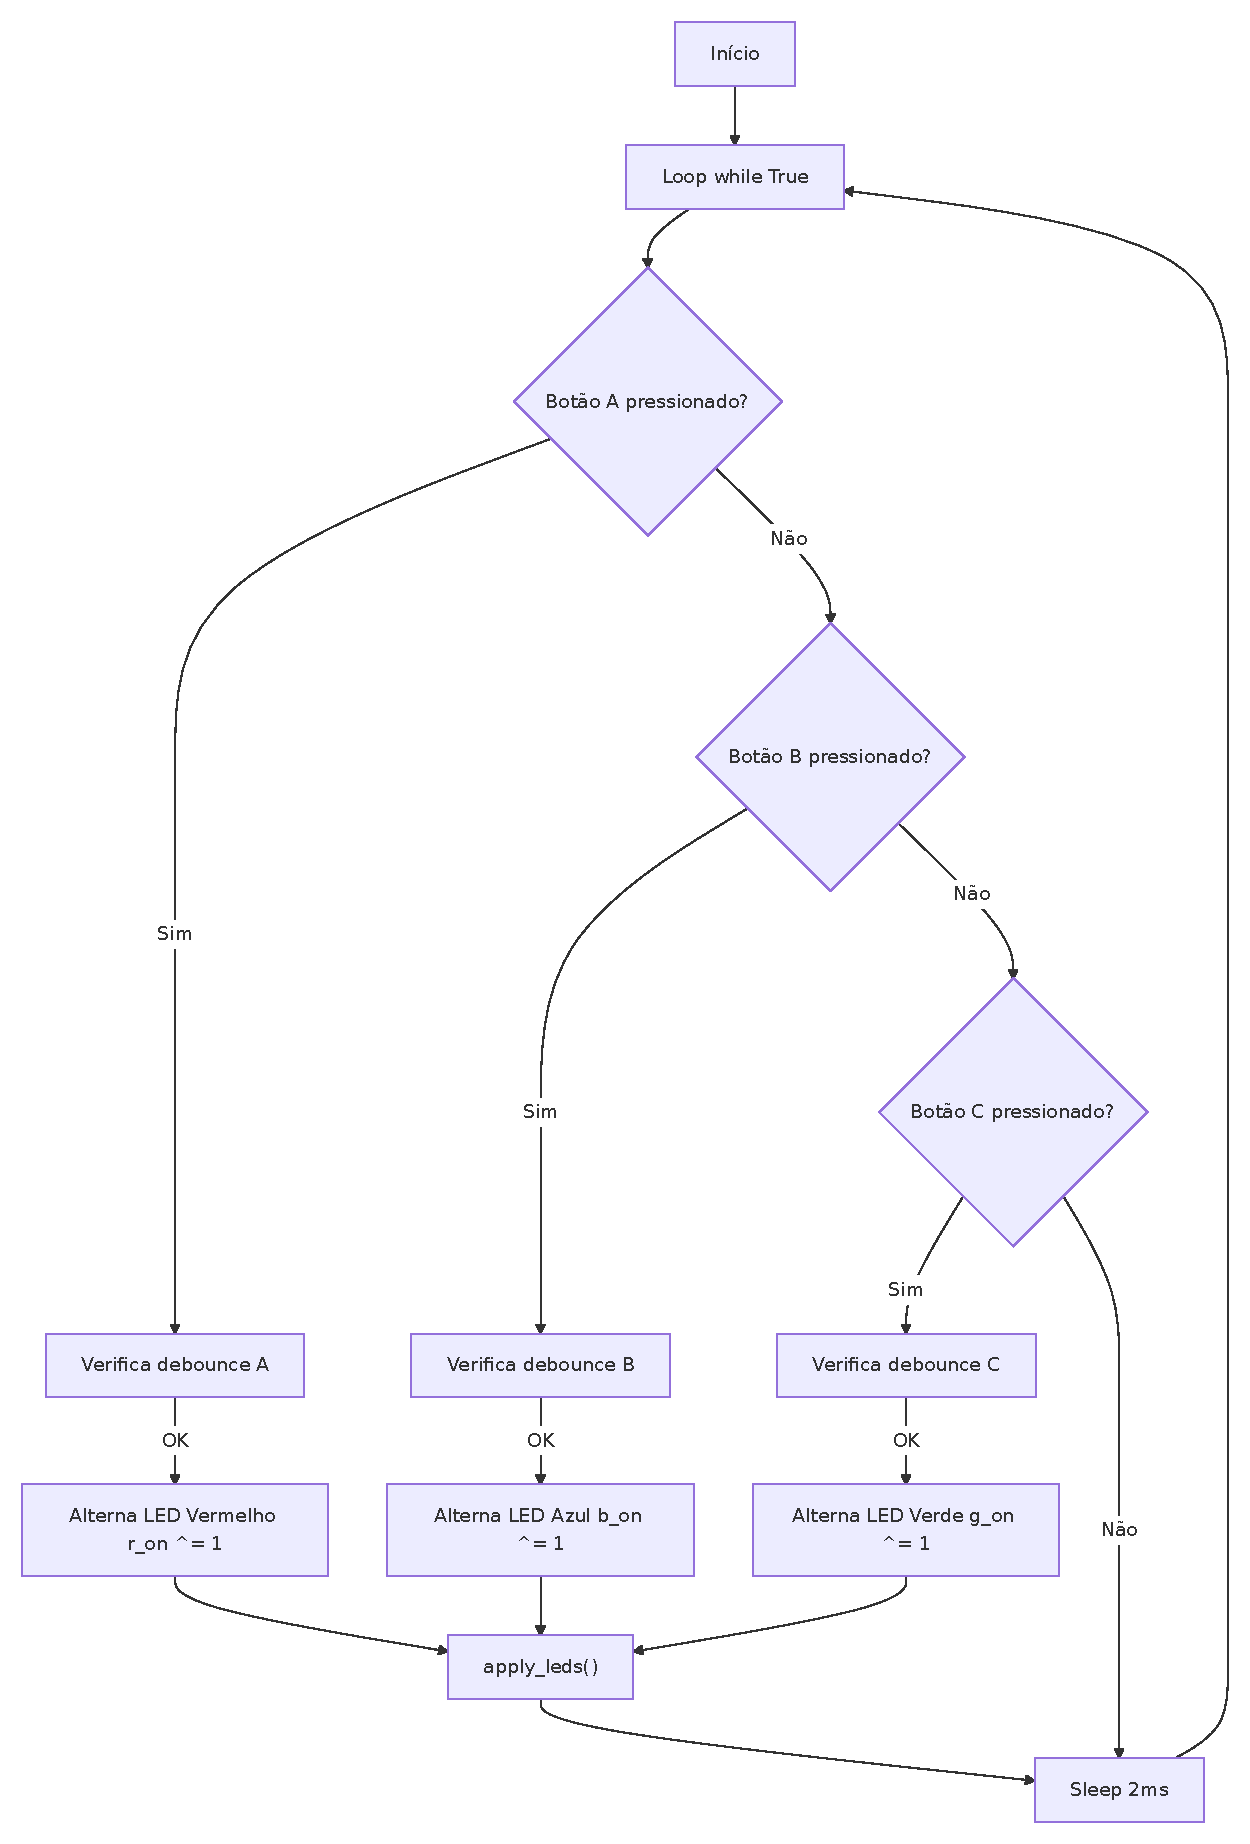
\includegraphics[width=\linewidth]{diagrama.pdf}
    \caption{Fluxograma do programa de toggle}
    \label{fig:togle}
\end{figure}

\subsection{Implementação e demonstração}
\noindent
\textbf{Pergunta:} Implementações em C e MicroPython (conforme códigos acima ou variações próprias). \\

\begin{lstlisting}[caption={Controle de LEDs com botões no Raspberry Pi Pico}]
#include "pico/stdlib.h"

#define PIN_R 12
#define PIN_G 13
#define PIN_B 11
#define BTN_A 5
#define BTN_B 6
#define BTN_C 10
#define DEBOUNCE_MS 40

int main() {
    stdio_init_all();

    gpio_init(PIN_R); gpio_set_dir(PIN_R, GPIO_OUT);
    gpio_init(PIN_G); gpio_set_dir(PIN_G, GPIO_OUT);
    gpio_init(PIN_B); gpio_set_dir(PIN_B, GPIO_OUT);

    gpio_init(BTN_A); gpio_set_dir(BTN_A, GPIO_IN); gpio_pull_up(BTN_A);
    gpio_init(BTN_B); gpio_set_dir(BTN_B, GPIO_IN); gpio_pull_up(BTN_B);
    gpio_init(BTN_C); gpio_set_dir(BTN_C, GPIO_IN); gpio_pull_up(BTN_C);

    bool r_on = false, g_on = false, b_on = false;
    bool lastA = true, lastB = true, lastC = true;
    absolute_time_t lastA_t = 0, lastB_t = 0, lastC_t = 0;

    while (true) {
        bool vA = gpio_get(BTN_A);
        bool vB = gpio_get(BTN_B);
        bool vC = gpio_get(BTN_C);
        absolute_time_t now = get_absolute_time();

        if (!vA && lastA) {
            if (absolute_time_diff_us(lastA_t, now) >= DEBOUNCE_MS * 1000) {
                r_on = !r_on;
                gpio_put(PIN_R, r_on);
                lastA_t = now;
            }
        }
        lastA = vA;

        if (!vB && lastB) {
            if (absolute_time_diff_us(lastB_t, now) >= DEBOUNCE_MS * 1000) {
                b_on = !b_on;
                gpio_put(PIN_B, b_on);
                lastB_t = now;
            }
        }
        lastB = vB;

        if (!vC && lastC) {
            if (absolute_time_diff_us(lastC_t, now) >= DEBOUNCE_MS * 1000) {
                g_on = !g_on;
                gpio_put(PIN_G, g_on);
                lastC_t = now;
            }
        }
        lastC = vC;

        sleep_ms(2);
    }
}
\end{lstlisting}


\noindent
\textbf{Pergunta:} Vídeo curto (link público) mostrando todas as combinações possíveis (R, G, B, RG, RB, GB, RGB). \\

\noindent
\textbf{Vídeo:} Disponível em: \url{https://youtube.com/shorts/5u4Is1JvaQc}

\subsection{Discução}

Neste caso em específico, a diferença entre usar C e MicroPython em termos de esforço de trabalho é muito pequena. Um programador já acostumado com C provavelmente acharia a implementação em Python menos prática, principalmente pela forma diferente como as coisas são estruturadas.

O debounce, nesta implementação, evita cliques múltiplos tanto no acionamento quanto no desligamento do botão. No entanto, o valor usado como exemplo (20 ms) é muito baixo; algo entre 50 e 150 ms seria mais adequado.

Além disso, o uso de IRQs eliminaria a necessidade do loop de varredura dos botões.

% ---------------- Conclusão ----------------
\section{Experimento 4}

\subsection{Gravação e demonstração}

\noindent
\textbf{Pergunta:} Testar e filmar o funcionamento (todas as combinações RGB). Inclua seu filme com um link público do youtube. \\

\noindent
\textbf{Vídeo:} Disponível em: \url{https://youtube.com/shorts/oYjkGLXbk-M}

\subsection{Comparação de simplicidade}

\noindent
\textbf{Pergunta:} Comparar: simplicidade do código em Python OO vs C modular com struct. \\

\noindent
A implementação em Python é consideravelmente mais legível e intuitiva do que em C com structs. No entanto, é possível adotar uma abordagem semelhante em C++, que, assim como o MicroPython, oferece suporte a classes, embora de forma mais verbosa.

Para desenvolvedores acostumados à forma como as coisas funcionam em C, a diferença em termos de simplicidade é mínima. \\

\noindent
\textbf{Pergunta:} Refletir: em quais casos o uso de IRQ + OO é vantajoso em sistemas embarcados reais (por ex.: interface homem-máquina, teclados matriciais, comunicação) \\

\noindent
Esta combinação, por si só, não traz vantagem significativa para o sistema. O uso de IRQs, por outro lado, acelera consideravelmente o tempo de resposta e otimiza a utilização da CPU. O uso de programação orientada a objetos (OO) pode facilitar a implementação de projetos maiores e mais complexos, mas exemplos de grande porte, como o Kernel Linux, o Zephyr e o ESP-IDF, demonstram que é possível organizar um projeto de forma estruturada sem recorrer obrigatoriamente à OO. \\

\subsection{Expansão da Abordagem}

\noindent
\textbf{Pergunta:} Como você adaptaria este mesmo programa se houvesse 10 botões (polling seria viável?) \\

Eu apenas adicionaria um case na função de callback para identificar qual GPIO foi pressionada e, com base nisso, executar a ação correspondente.

O polling pode ser viável dependendo da carga de trabalho adicional. Vale lembrar que teclados antigos, como o BTC 5339-R, que utilizam o microcontrolador Intel 8049, funcionavam justamente por varredura. Para microcontroladores modernos, como o Raspberry Pi Pico, que operam na faixa de MHz, monitorar 10 GPIOs via polling seria uma tarefa trivial, quase como caminhar em um planalto.

\end{document}
